\documentclass{report}
\usepackage[utf8]{inputenc}
\usepackage{amsmath, amssymb}
\usepackage{graphicx}
\usepackage[margin=1.25in]{geometry}
\usepackage{multirow}
\usepackage{pdfpages}
\usepackage{float}
\usepackage{hyperref}
\hypersetup{
    colorlinks,
    citecolor=black,
    filecolor=black,
    linkcolor=black,
    urlcolor=black
}
\title{Lab \#5: Diffraction \& Interference}
\author{Neil Sawhney}
\date{December 2021}

\makeatletter
\def\@makechapterhead#1{%
  \vspace*{50\p@}% <----------------- Space from top of page to Chapter #
  {\parindent \z@ \raggedright \normalfont
    \ifnum \c@secnumdepth >\m@ne
        \huge\bfseries \thechapter.\ % <-- Chapter # (without "Chapter")
    \fi
    \interlinepenalty\@M
    #1\par\nobreak% <------------------ Chapter title
    \vskip 40\p@% <------------------ Space between chapter title and first paragraph
  }}
\makeatother
\begin{document}

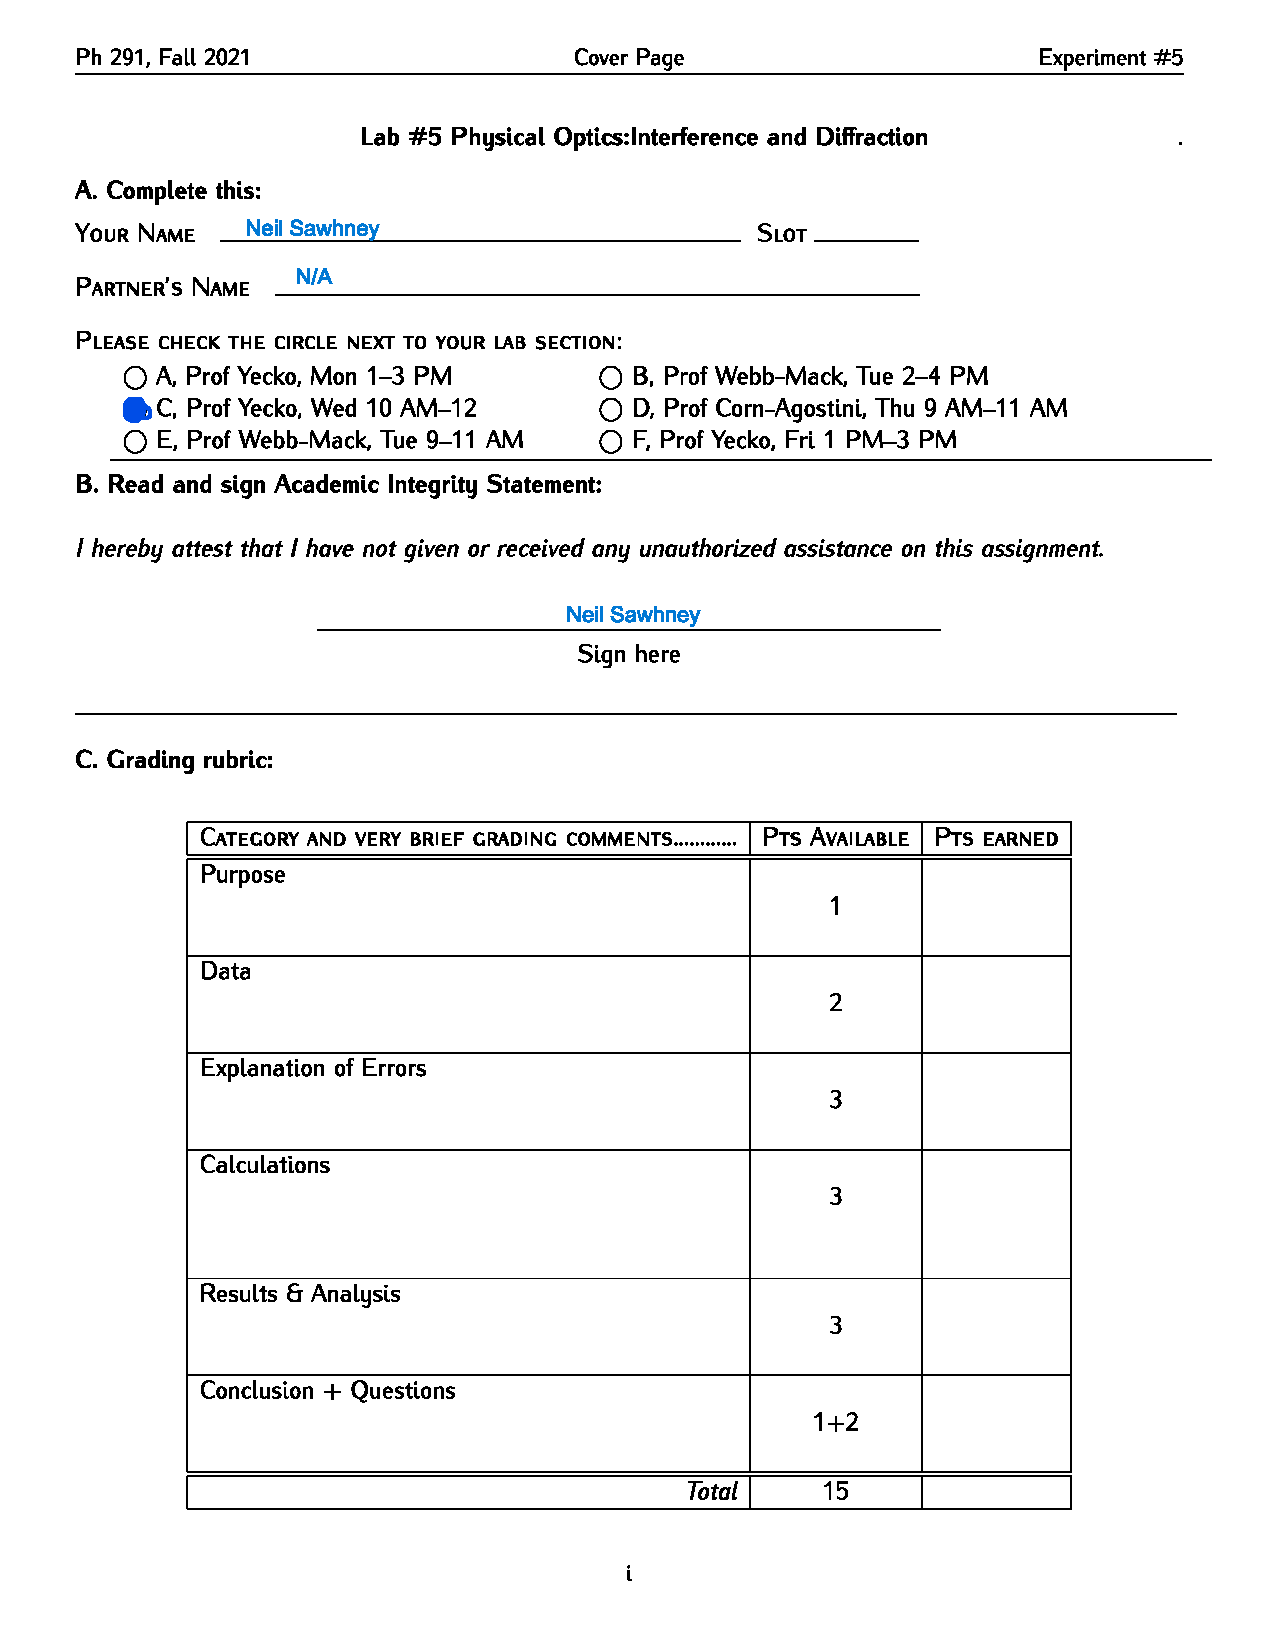
\includepdf[pages=-]{Lab5_Cover.pdf}

\maketitle
\tableofcontents

\chapter{Purpose}
The purpose of this lab is to determine the wavelength of a red laser pointer and the thickness of a human hair by using the interference pattern created due to the wave like nature of light.


%-----------------------------------

\chapter{Data}

\begin{table}[H]
    \centering
    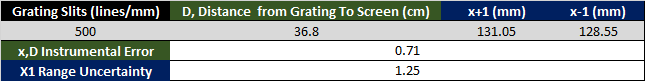
\includegraphics[width = \textwidth]{partATable.png}
    \caption{Diffraction Grating}
    \label{partATable}
\end{table}
\bigskip


\begin{table}[H]
    \centering
    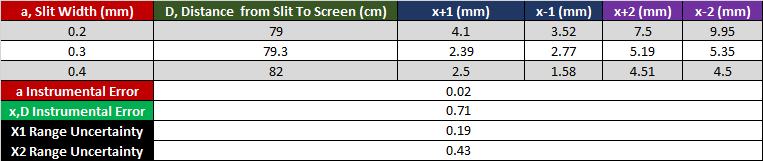
\includegraphics[width = \textwidth]{partBTable.png}
    \caption{Single Slit}
    \label{partBTable}
\end{table}
\bigskip


\begin{table}[H]
    \centering
    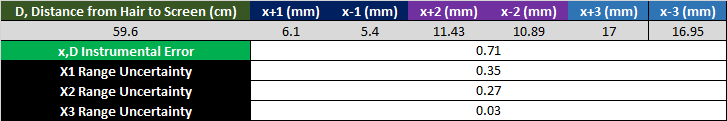
\includegraphics[width = \textwidth]{partCTable.png}
    \caption{Hair Reverse Slit}
    \label{partCTable}
\end{table}
\bigskip



\chapter{Sources of uncertainty}
\begin{itemize}
    \item center of dots were roughly estimated, since the edges were fuzzy and the circles were large
    \item center of lines were roughly estimated, since the edges were fuzzy and the lines were long
    \item center of lines were roughly estimated, since the edges were fuzzy and the lines were long
\end{itemize}

\chapter{Calculations}

\section{Wavelength Calculations}
\subsection*{Part A}

\subsubsection*{Value}
%maths
\begin{equation}
    I(\delta)=I_{0}\left[\frac{\sin \left(\frac{N \delta}{2}\right)}{\sin \left(\frac{\delta}{2}\right)}\right]^{2} \text { where } \delta \equiv \frac{2 \pi}{\lambda} d \sin \theta 
\end{equation}
\label{Question}

\subsection*{Question}
$$
\lim
$$
$$
    \sin \theta=\frac{m \lambda}{d} \quad m=0, \pm 1, \pm 2, \ldots
$$

$$
\begin{gathered}
    \tan \theta  = \frac{\text{Average of $x_m$}}{D} \\
    \theta = \arctan \left( \frac{\text{Average of $x_m$}}{D} \right) \\
    \lambda = \frac{d}{m}\sin \left(\arctan \left( \frac{\text{Average of $x_m$}}{D} \right)\right) \\
    d = \frac{1 \ mm}{500 \ lines} * 1 \ lines = 0.002 mm \\
    \lambda = 0.002*10^{-3}\sin \left(\arctan \left( \frac{(131.05 * 10^{-3} + 128.55*10^{-3}) / 2}{36.8*10^{-2}} \right)\right) \quad \text{where m} = \pm 1 \\
    \lambda = 0.002*10^{-3}\sin \left(\arctan \left( \frac{(131.05 * 10^{-3} + 128.55*10^{-3}) / 2}{36.8*10^{-2}} \right)\right) \\
    \lambda = 6.6526*10^{-7}  \ \mathrm{m} = 665.26 \  \mathrm{nm} \\
\end{gathered}
$$

\subsubsection*{Error}
%maths
$$
\begin{gathered}
    \lambda = \frac{d}{m}\sin \left(\arctan \left( \frac{(x_{+1} + x_{-1}) /2}{D} \right)\right) \\
    \delta \lambda=\left|\frac{\partial \lambda}{\partial D} * \delta D\right|+\left|\frac{\partial \lambda}{\partial x_{+1}} * \delta x_{+1}\right|+ \left|\frac{\partial \lambda}{\partial x_{-1}} * \delta x_{-1}\right| \\
    \begin{aligned}
    \delta \lambda=&\left|-\frac{4dD\left(x_{+1}+x_{-1}\right)}{m\left(\left(x_{+1}+x_{-1}\right)^2+4D^2\right)\sqrt{4D^2+\left(x_{+1}+x_{-1}\right)^2}} * \delta D\right|+ \\
    &\left|\frac{4dD^2}{m\left(\left(x_{+1}+x_{-1}\right)^2+4D^2\right)\sqrt{4D^2+\left(x_{+1}+x_{-1}\right)^2}} * \delta x_{+1}\right|+  \\
    &\left|\frac{4dD^2}{m\left(\left(x_{-1}+x_{+1}\right)^2+4D^2\right)\sqrt{4D^2+\left(x_{+1}+x_{-1}\right)^2}} * \delta x_{-1}\right| \\
    \delta \lambda=&\left|-\frac{(0.008)(0.368)\left(131.05+128.55\right)}{\left(\left(131.05+128.55\right)^2+4(0.368)^2\right)\sqrt{4(0.368)^2+\left(131.05+128.55\right)^2}} * 0.71\right|+ \\
    &\left|\frac{(0.008)(0.368)^2}{\left(\left(131.05+128.55\right)^2+4(0.368)^2\right)\sqrt{4(0.368)^2+\left(131.05+128.55\right)^2}} *1.25\right|+  \\
    &\left|\frac{(0.008)(0.368)^2}{\left(\left(128.55+131.05\right)^2+4(0.368)^2\right)\sqrt{4(0.368)^2+\left(131.05+128.55\right)^2}} *1.25\right| \\
    \delta \lambda=&\frac{1065107 \sqrt{263252741}}{554416045152104648 }= \pm 3.1170*10^{-8} \ \mathrm{m} = \pm 30 \ \mathrm{nm}     \end{aligned} \\
\end{gathered}
$$


\subsection*{Part B}

\subsubsection*{Value}
%maths
$$
\begin{gathered}
I(\beta)=I_{0}\left(\frac{\sin \beta}{\beta}\right)^{2} \quad \text { where } \beta \equiv \frac{\pi}{\lambda} a \sin \theta \\
\sin \theta=\frac{p \lambda}{a} \quad p=\pm 1, \pm 2, \ldots \\
\sin \theta=\frac{p \lambda}{a}\\
\lambda_n=\frac{\sin \left(\theta\right)a}{p} \\
\lambda_n=\frac{\sin \left(\arctan \left( \frac{\text{Average of $x_p$}}{D} \right)\right)a}{p} \\
\lambda_1=\frac{\sin \left(\arctan \left( \frac{(4.1(10^{-3})+3.52(10^{-3}))/2}{79(10^{-2})} \right)\right)0.2(10^{-3})}{1} 9.6454(10^-7) \ \mathrm{m} = 964.54 \ \mathrm{nm} \\
\lambda = \frac{1}{6}\sum_{n = 1}^{n = 6} \lambda_n \\
\lambda = \frac{1}{6}{\left(964.54 + 1104.36 + 976.04 + 996.83 +  995.12 + 1098.76\right)}=1022.608 \  \mathrm{nm}\\
\end{gathered}
$$

\subsubsection*{Error}
%maths

$$
\begin{gathered}
    \lambda_n=\frac{\sin \left(\arctan \left( \frac{(x_{+p} + x_{-p})/2}{D} \right)\right)a}{P} \\
    %
    \delta \lambda=\left|\frac{\partial \lambda}{\partial D} * \delta D\right|+\left|\frac{\partial \lambda}{\partial x_{+p}} * \delta x_{+p}\right|+ \left|\frac{\partial \lambda}{\partial x_{-p}} * \delta x_{-p}\right|+ \left|\frac{\partial \lambda}{\partial a} * \delta a\right|\\
    %
    \delta \lambda=\left|-\frac{4aD\left(x_{+p}+x_{-p}\right)}{P\left(\left(x_{+p}+x_{-p}\right)^2+4D^2\right)\sqrt{4D^2+\left(x_{+p}+x_{-p}\right)^2}}* \delta D\right|+ \\
    \left|\frac{4aD^2}{P\left(\left(x_{+p}+x_{-p}\right)^2+4D^2\right)\sqrt{4D^2+\left(x_{+p}+x_{-p}\right)^2}} * \delta x_{+p}\right|+ \\ 
    \left|\frac{4aD^2}{P\left(\left(x_{-p}+x_{+p}\right)^2+4D^2\right)\sqrt{4D^2+\left(x_{+p}+x_{-p}\right)^2}} * \delta x_{-p}\right|+ \\
    \left|\frac{x_{+p}+x_{-p}}{P\sqrt{4D^2+\left(x_{+p}+x_{-p}\right)^2}} * \delta a\right|\\
%
    \delta \lambda=\left|-\frac{4(0.2)(790)\left(4.1+3.52\right)}{1\left(\left(4.1+3.52\right)^2+4(790)^2\right)\sqrt{4(790)^2+\left(4.1+3.52\right)^2}}* 0.71 \right|+ \\ \left|\frac{4(0.2)(790)^2}{1\left(\left(4.1+3.52\right)^2+4(790)^2\right)\sqrt{4(790)^2+\left(4.1+3.52\right)^2}} * 0.71\right|+ \\ \left|\frac{4(0.2)(790)^2}{1\left(\left(3.52+4.1\right)^2+4(790)^2\right)\sqrt{4(790)^2+\left(4.1+3.52\right)^2}} * 0.71\right|+ \\ \left|\frac{4.1+3.52}{1\sqrt{4(790)^2+\left(4.1+3.52\right)^2}} * 0.02\right| = 2.770 * 10^{-7} \ \mathrm{m} \\
    \delta \lambda = \pm 277 \ \mathrm{nm}
\end{gathered}
$$

\section{Hair Thickness Calculations}

\subsubsection*{Value}
%maths
$$
\begin{gathered}
\lambda_n=\frac{\sin \left(\arctan \left( \frac{(x_{+p} + x_{-p})/2}{D} \right)\right)a}{P} \\
a_1 = \frac{\lambda_n  P}{\sin \left(\arctan \left( \frac{(x_{+p} + x_{-p})/2}{D} \right)\right)} \\
a_1 = \frac{(660 * 10^{-9})(1)}{\sin \left(\arctan \left( \frac{(6.1*10^{-3} + 5.4*10^{-3})/2}{59.6*10^{-2}} \right)\right)} \\
=6.84*10{-5} \ \mathrm{m} = 68.4 \ \mathrm{\mu m}  \\
a_2  = \frac{(660 * 10^{-9})(2)}{\sin \left(\arctan \left( \frac{(11.43*10^{-3} + 10.89*10^{-3})/2}{59.6*10^{-2}} \right)\right)} =7.050*10^{-5} \ \mathrm{m} = 70.5 \ \mathrm{\mu m}\\
a_3  = \frac{(660 * 10^{-9})(2)}{\sin \left(\arctan \left( \frac{(17*10^{-3} + 16.95*10^{-3})/2}{59.6*10^{-2}} \right)\right)} =4.636*10^{-5} \ \mathrm{m} = 46.4 \ \mathrm{\mu m} \\
a = (a_1 + a_2 + a_3)/3 =  (68.4 + 70.5 + 46.4)/3=61.76 \\
\end{gathered}
$$

\subsubsection*{Error}
%maths
$$
\begin{gathered}
    a = \frac{\lambda_n  P}{\sin \left(\arctan \left( \frac{(x_{+p} + x_{-p})/2}{D} \right)\right)} \\
%
    \delta a=\left|\frac{\partial a}{\partial D} * \delta D\right|+\left|\frac{\partial a}{\partial x_{+p}} * \delta x_{+p}\right|+ \left|\frac{\partial a}{\partial x_{-p}} * \delta x_{-p}\right|+ \left|\frac{\partial a}{\partial \lambda} * \delta \lambda\right|\\
%
    \delta a=\left|\frac{4\lambda PD}{\left(x_1+x_2\right)\sqrt{4D^2+\left(x_1+x_2\right)^2}} * \delta D\right|+\\\left|-\frac{4\lambda PD^2}{\left(x_1+x_2\right)^2\sqrt{4D^2+\left(x_1+x_2\right)^2}} * \delta x_{+p}\right|  + \\ \left|-\frac{4\lambda PD^2}{\left(x_1+x_2\right)^2\sqrt{4D^2+\left(x_1+x_2\right)^2}} * \delta x_{-p}\right|  + \\ \left|\frac{P\sqrt{4D^2+\left(x_1+x_2\right)^2}}{x_1+x_2} * \delta \lambda\right|\\
%
    \delta a=\left|\frac{4(660 * 10^{-9}) 1(59.6 * 10^{-2})}{\left(6.1+5.4\right)\sqrt{4(59.6 * 10^{-2})^2+\left(6.1+5.4\right)^2}} * (0.71)\right|+\\\left|-\frac{4(660 * 10^{-9}) 1(59.6 * 10^{-2})^2}{\left(6.1+5.4\right)^2\sqrt{4(59.6 * 10^{-2})^2+\left(6.1+5.4\right)^2}} * (0.71)\right|  + \\ \left|-\frac{4(660 * 10^{-9}) 1(59.6 * 10^{-2})^2}{\left(6.1+5.4\right)^2\sqrt{4(59.6 * 10^{-2})^2+\left(6.1+5.4\right)^2}} * (0.71 )\right|  + \\ \left|\frac{1\sqrt{4(59.6 * 10^{-2})^2+\left(6.1+5.4\right)^2}}{6.1+5.4} * (30 * 10^{-9})\right|\\ = 3.94338174505277*10^{-8} \ \mathrm{m} = .04 \ \mathrm{\mu m}
\end{gathered}
$$



\chapter{Results}

\section*{Wavelength}
\subsection*{Part A}
\begin{equation*}
    \begin{aligned}
        \text{Calculated Wavelength} & = 660 \pm 30 \ \mathrm{nm} \\
    \end{aligned}
\end{equation*}

\subsection*{Part B}
\begin{equation*}
    \begin{aligned}
        \text{Calculated Wavelength} & = 1000 \pm 300 \ \mathrm{nm} \\
    \end{aligned}
\end{equation*}

\section*{Hair Thickness}
\begin{equation*}
    \begin{aligned}
        \text{Calculated Hair Thickness} & = 61.76 \pm 0.04 \ \mathrm{\mu m} \\
    \end{aligned}
\end{equation*}



\chapter{Conclusions}

By using the interference and wave like nature of light, the diffraction pattern created by a laser hitting a hair was used to determine the thickness of the hair. The error bounds of the calculated value agrees with literature values.  




\chapter{Answered Questions}
Click the question to be brought to the location where the question is answered.

\section{Question}
\hyperref[Question]{Derivation for Principal Maxima}

\end{document}
